% Asset ID: A22StatisticalHypothesisTestingTIKZ-005
% Unit code: A22
% Topic code: A22-HT
% Topic name: Statistical hypothesis testing
% Related lesson section: Core Theory, What regression means
% Source: Lesson transcript and Stats Yr2 Chapter 1 PDF
% Purpose: Show how the fitted regression line is compared with data points using vertical gaps.
% Status: Phase 4 TikZ draft

\documentclass[tikz,border=8pt]{standalone}
\usepackage{amsmath}
\usepackage{tikz}
\usetikzlibrary{arrows.meta}
\begin{document}
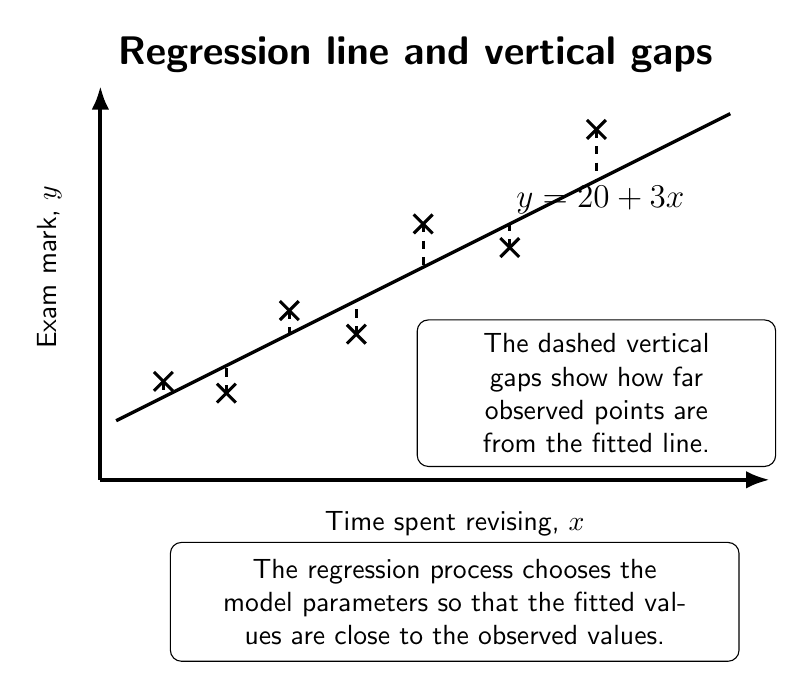
\begin{tikzpicture}[font=\sffamily,axis/.style={line width=1.4pt,-{Latex[length=3mm]}},point/.style={line width=1.1pt},residual/.style={line width=1pt,dashed}]
\node[font=\sffamily\bfseries\Large] at (4,5.4){Regression line and vertical gaps};
\draw[axis] (0,0) -- (8.5,0); \draw[axis] (0,0) -- (0,5);
\node at (4.5,-0.55) {Time spent revising, \(x\)}; \node[rotate=90] at (-0.65,2.7) {Exam mark, \(y\)};
\draw[line width=1.2pt] (0.2,0.75) -- (8.0,4.65); \node[font=\sffamily\large] at (6.35,3.55) {\(\displaystyle y=20+3x\)};
\foreach \x/\y/\yf in {0.8/1.25/1.05,1.6/1.10/1.45,2.4/2.15/1.85,3.25/1.85/2.28,4.1/3.25/2.70,5.2/2.95/3.25,6.3/4.45/3.80} {\draw[residual] (\x,\y) -- (\x,\yf); \draw[point] (\x-0.12,\y-0.12) -- (\x+0.12,\y+0.12); \draw[point] (\x-0.12,\y+0.12) -- (\x+0.12,\y-0.12);}
\node[draw,rounded corners=4pt,text width=6.8cm,align=center,inner sep=6pt] at (4.5,-1.55){The regression process chooses the model parameters so that the fitted values are close to the observed values.};
\node[draw,rounded corners=4pt,text width=4.2cm,align=center,inner sep=5pt] at (6.3,1.1){The dashed vertical gaps show how far observed points are from the fitted line.};
\end{tikzpicture}
\end{document}
